% ══════════════════════════════════════════════════════════════════════════════
%  CHAPTER 1: BASICS CONCEPTS IN ASTROPHYSICS
% ══════════════════════════════════════════════════════════════════════════════
\chapter{Basic Concepts in Astrophysics}
Astrophysics is the branch of astronomy that applies the principles of physics and chemistry to understand the nature of celestial objects and phenomena. It includes but is not limited to the study of stars, galaxies, extrasolar planets, cosmic microwave background radiation, and the interstellar medium. In this notes, we will only focus on the field of stellar astrophysics, which is the study of stars, their properties, structure, types, and evolution.
% ═════════════════════════════════════════════════════════════════════════════ 
\bigskip\noindent 
\section{Stars and Stellar Properties}
\begin{intuition}
    In this notes, we define a star as a celestial object that is:
    \begin{itemize}
        \item (1) bounded by self-gravity under hydrostatic equilibrium, and
        \item (2) radiating energy generated by internal sources (e.g. nuclear fusion). 
    \end{itemize}
    For most of the case, a star is spherical due to spherical symmetry of gravity, and mainly radiating energy by nuclear fusion in the core. However, we will also encounter some exceptions (e.g. energy generated by gravitational contraction in late stages of star evolution). \\

    This definition shows that other celestial objects (e.g. planets, comets) are not stars as they don't fulfill all conditions. On the other hand, it allow some special conditions (e.g. brown dwarfs, white dwarfs) to be classified as stars, as they are still self-gravitating and radiating energy (though not by nuclear fusion). However, be careful some astrophysicists may not treat them as "real stars" as they don't have nuclear fusion, but we will still include them in our discussion as they are important for understanding the full picture of stellar evolution.
\end{intuition}

\begin{remark}
The stars are usually of spherical shape due to rotational symmetric force field of gravity, but can be oblate if they rotate rapidly.
\end{remark}

% ---------------------------------------------------------------------------------
\bigskip\noindent \bigskip\noindent \bigskip\noindent
\subsection{Distance and Parallax}
\begin{intuition}
    Parallax is the apparent shift in position of a nearby star against the background of distant stars when observed from different positions (e.g. Earth at different points in its orbit). By measuring this shift, we can determine the distance to the star using simple trigonometry.
\end{intuition}

\begin{figure}[ht]
    \centering
    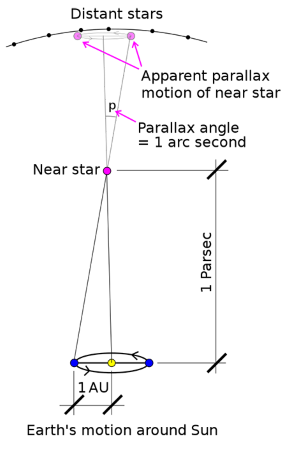
\includegraphics[height=0.3\textheight,width=0.35\textwidth]{images/stellar_parallax.png}
    \caption{Stellar parallax illustration. The nearby star appears to shift position against the background of distant stars as Earth orbits the Sun. The angle $p$ is the shifted angle actually, instead of the parallex angle $\frac{1}{2}p$.}
    \label{fig:stellar_parallax}
\end{figure}


\begin{theory}
    Let x be the baseline (e.g. diameter of Earth's orbit), d be the distance to the star, and $\theta$ be the parallax angle (half of the shifted angle $p$). Then we have:
    \begin{itemize}
        \item Parallax distance:
        \begin{equation}
            d_{\text{pc}} = \tan^{-1}\left(\frac{x/2}{d}\right) \approx \frac{1 \text{AU}}{\theta_{\text{arcsec}}}
        \end{equation}

        \item we can also directly calculate the radius of the star if we know its angular radius $\theta$ and distance $d$:
        \begin{equation}
            R = d \dot \tan\theta \approx d \theta
        \end{equation}
    \end{itemize}
\end{theory}

\begin{importantnote}
    Don't mixed up the parallax angle $\theta$ and the shifted angle $p$ in the parallax measurement. The total shifted angle $p$ shows the apparent shift of the star, but when we use the trigonometry to calculate the distance, we need to use the parallax angle $\theta = \frac{1}{2}p$ which is the angle between the line of sight to the star and the line connecting the Earth and the Sun. 
\end{importantnote}

\begin{example}{}{ex:distmod1}
    From the previous example, if the star has an angular diameter of $0.01$ arcseconds, estimate its radius in units of $R_\odot$.

    \smallskip\textbf{Solution.}
    \begin{align*}
    R &= \frac{1}{2}\theta d = \frac{1}{2} \times 0.01'' \times 100\,\text{pc} \\
    &= 0.5 \times 0.01 \times 100 \times 206265\,\text{AU} \\
    &= 1031.325\,\text{AU} \\   
    &= 1031.325 \times 215 R_\odot \\
    &\approx 221,000 R_\odot.
    \end{align*}
\end{example}

\begin{example}{}{ex:distmod2}
    Assume a telescope angular resolution of $0.01$ arcseconds. \\
    (a). what is the maximum distance at which we can resolve a star with a radius of $R_\odot$? \\
    (b). If baseline $x$ is $2$ AU, what is the maximum distance of a star we can resolve?

    \smallskip\textbf{Solution.}
    (a). We can use the formula for the radius of the star:
        \begin{align*}
            R &\geq d \theta \\
            d &\leq \frac{R}{\theta} = \frac{R_\odot}{0.01''} \\
        \end{align*}
        As $R_\odot \approx 6.957 \times 10^8$ m and $1'' = 4.848 \times 10^{-6}$ radians, we have:
        \begin{align*}
            d &\leq \frac{6.957 \times 10^8\,\text{m}}{0.01 \times 4.848 \times 10^{-6}} \\
            &\approx 1.43 \times 10^{16}\,\text{m} \\
            &\approx 0.465\,\text{pc}.
        \end{align*}
    (b). Using the parallax distance formula:
        \begin{align*}
            d &\leq \frac{x/2}{\tan\theta} \approx \frac{1\,\text{AU}}{0.01''} \\
            &\approx 100\,\text{pc}.
        \end{align*}
\end{example}

\begin{remark}
    As we can see from the above examples, the stellar parallax method is only effective for measuring distances to nearby stars (within a few hundred parsecs). For more distant stars, we need to use other methods such as spectroscopic parallax or standard candles.(we will discuss these methods in later chapters).
\end{remark}

% ---------------------------------------------------------------------------------
\bigskip\noindent \bigskip\noindent \bigskip\noindent
\subsection{Brightness, Magnitude, and Luminosity}
\begin{theory}
\begin{align}
    M_1 - M_2 &= -2.5 \log_{10}\left(\frac{L_1}{L_2}\right), \\
    m_1 - m_2 &= -2.5 \log_{10}\left(\frac{F_1}{F_2}\right), \\
    m - M &= 5 \log_{10}(d/\text{pc}) - 5, \\
    F &= \frac{L}{4\pi d^2}.
\end{align}
\end{theory}

\begin{example}{Distance modulus quick use}{ex:distmod}
A star has $m=9.0$ and $M=4.0$. Estimate its distance.

\smallskip\textbf{Solution.}
\begin{align*}
m-M &= 5\log_{10}(d/\text{pc})-5 = 5 \\
\Rightarrow \log_{10}(d/\text{pc}) &= 2 \\
\Rightarrow d &= 10^2\,\text{pc} = 100\,\text{pc}.
\end{align*}
\end{example}

% ---------------------------------------------------------------------------------
\bigskip\noindent \bigskip\noindent \bigskip\noindent
\subsection{Mass}

% ═════════════════════════════════════════════════════════════════════════════ 
\bigskip\noindent \bigskip\noindent \bigskip\noindent
\section{Thermal Radiation and Blackbody Spectrum}
% ---------------------------------------------------------------------------------
\bigskip\noindent \bigskip\noindent \bigskip\noindent
\subsection{Planck function, Rayleigh-Jeans law, Wien's law}
\begin{theory}
\begin{itemize}
    \item Planck function:
    \begin{equation}
        B_\nu(T) = \frac{2h\nu^3}{c^2}\frac{1}{e^{h\nu/k_B T}-1}
    \end{equation}
    \item Stefan--Boltzmann law:
    \begin{equation}
        F = \sigma T^4, \quad \sigma = \SI{5.67e-8}{\watt\per\square\meter\per\kelvin\tothe{4}}
    \end{equation}
    \item Luminosity:
    \begin{equation}
        L = 4\pi R^2 \sigma T_{\text{eff}}^4
    \end{equation}
    \item Wien's law:
    \begin{equation}
        \lambda_{\text{max}}T = \SI{2.9e-3}{\meter\kelvin}
    \end{equation}
\end{itemize}
\end{theory}
\begin{example}{}{ex:wien}
A star has a peak wavelength of $500\,\text{nm}$. Estimate its surface temperature.

\smallskip\textbf{Solution.}
From Wien's law,
\begin{align*}
    \lambda_{\text{max}} T &= 2.9 \times 10^{-3}\,\text{m K} \\
    T &= \frac{2.9 \times 10^{-3}\,\text{m K}}{\lambda_{\text{max}}} \\
    &= \frac{2.9 \times 10^{-3}\,\text{m K}}{500 \times 10^{-9}\,\text{m}} \\
    &= 5800\,\text{K}.
\end{align*}
\end{example}

% ---------------------------------------------------------------------------------
\bigskip\noindent \bigskip\noindent \bigskip\noindent
\subsection{Intensity, Flux, and Luminosity}
\begin{intuition}
Observed starlight is measured in layers: direction-resolved intensity, surface flux, and finally total emitted power.
Keeping these definitions separate avoids unit mistakes in later derivations.
\end{intuition}

\begin{theory}
\begin{itemize}
    \item Specific intensity $I_\nu$:
    \begin{equation}
        dE = I_\nu \cos\theta \, dA \, dt \, d\nu \, d\Omega
    \end{equation}
    \item Monochromatic flux density:
    \begin{equation}
        F_\nu = \int I_\nu \cos\theta \, d\Omega
    \end{equation}
    \item Bolometric flux:
    \begin{equation}
        F = \int_0^\infty F_\nu \, d\nu
    \end{equation}
    \item Luminosity:
    \begin{equation}
        L = \int F \, dA
    \end{equation}
\end{itemize}
\end{theory}

\begin{importantnote}
$I_\nu$ is invariant along a ray in vacuum (no absorption/emission), while $F_\nu$ depends on source geometry and distance.
Do not interchange them in magnitude or distance calculations.
\end{importantnote}

% ---------------------------------------------------------------------------------
\bigskip\noindent \bigskip\noindent \bigskip\noindent
\subsection{Radiative Transfer}

\begin{example}{Calculating Brightness}{ex:brightness}
Suppose a star is at 20 pc. How bright does it appear if its luminosity is $100 L_\odot$?
\smallskip\textbf{Solution.}
\begin{align*}
F &= \frac{L}{4\pi d^2} = \frac{100 L_\odot}{4\pi (20\,\text{pc})^2} \\
&= \frac{100 \times 3.828 \times 10^{26}\,\text{W}}{4\pi (20 \times 3.086 \times 10^{16}\,\text{m})^2} \\
&\approx 3.1 \times 10^{-9}\,\text{W/m}^2.
\end{align*}
\end{example}

% ---------------------------------------------------------------------------------
\bigskip\noindent \bigskip\noindent \bigskip\noindent
\subsection{Surface Temperature}

\section{Surface Temperature and Spectral Classification}
Recall that the surface temperature $T_{\text{eff}}$ of a star can be estimated from its luminosity and radius using the Stefan-Boltzmann law:
\begin{equation}
L = 4\pi R^2 \sigma T_{\text{eff}}^4
\end{equation}
where $\sigma$ is the Stefan-Boltzmann constant. Rearranging this gives:
\begin{equation}
T_{\text{eff}} = \left(\frac{L}{4\pi R^2 \sigma}\right)^{1/4}
\end{equation}
\begin{example}{Estimating Surface Temperature}{ex:estimating_surface_temperature}
A star has a luminosity of $300 L_\odot$ and a radius of $25 R_\odot$. Estimate its surface temperature.

\smallskip\textbf{Solution.}
First, we need to convert the luminosity and radius into SI units:
\begin{align*}
L &= 300 L_\odot = 300 \times 3.828 \times 10^{26}\,\text{W} = 1.1484 \times 10^{29}\,\text{W}, \\
R &= 25 R_\odot = 25 \times 6.957 \times 10^8\,\text{m} = 1.73925 \times 10^{10}\,\text{m}.
\end{align*}
Now we can plug these values into the formula for $T_{\text{eff}}$:
\begin{align*}
T_{\text{eff}} &= \left(\frac{1.1484    \times 10^{29}\,\text{W}}{4\pi (1.73925 \times 10^{10}\,\text{m})^2 \times 5.67 \times 10^{-8}\,\text{W/m}^2\text{K}^4}\right)^{1/4} \\
&\approx 4500\,\text{K}.
\end{align*}
\end{example}


\subsection{Spectral Classification}
Apart from direct use of $L$, we can also estimate $T_{\text{eff}}$ from the star's spectral type, which is determined by its surface temperature and spectral features. 
\begin{theory}
Stars are classified into spectral types O, B, A, F, G, K, M based on their surface temperatures and spectral features. O-type stars are the hottest and most massive, while M-type stars are the coolest and least massive.
Each spectral type corresponds to a specific range of surface temperatures, which can be used to estimate $T_{\text{eff}}$ if the spectral type is known.
\end{theory}





